\documentclass[xcolor=dvipsnames,aspectratio=169]{beamer}
\usepackage[utf8]{inputenc}
\usetheme{Warsaw}
\usepackage{pgfpages}

% -----------------------------------------------------------------------------
% Notes toggle
% Compile with \def\NOTES{} before \input if you want notes-only output.
% -----------------------------------------------------------------------------
\newif\ifnotes
\ifdefined\NOTES\notestrue\fi
\ifnotes
  \setbeameroption{show only notes}
\else
  \setbeameroption{hide notes}
\fi

% -----------------------------------------------------------------------------
% Shared formatting
% -----------------------------------------------------------------------------
\setcounter{tocdepth}{2}

% =============================================================================
% Theme settings
% =============================================================================

% --- Core theme colors ---
\definecolor{ThemePrimary}{rgb}{0.0745, 0.1608, 0.2941}   % deep blue
\definecolor{ThemeSecondary}{rgb}{0.8667, 0.2039, 0.0118} % warm red/orange
\definecolor{ThemeAccent}{rgb}{0.1137, 0.3451, 0.6549}    % medium blue
\definecolor{ThemeLight}{rgb}{0.9725, 0.9804, 0.9882}     % near white
\definecolor{ThemeText}{rgb}{0.10, 0.10, 0.10}

% --- Optional extra palette ---
\definecolor{ThemeHighlight}{rgb}{0.9608, 0.5294, 0.1176}
\definecolor{ThemeSoftBlue}{rgb}{0.0000, 0.6235, 0.8314}
\definecolor{ThemeSoftNavy}{rgb}{0.1176, 0.2196, 0.4667}

% =============================================================================
% Beamer color settings
% =============================================================================

\setbeamercolor{palette primary}{bg=ThemePrimary,fg=ThemeLight}
\setbeamercolor{structure}{fg=ThemePrimary}
\setbeamercolor{section in toc}{fg=ThemePrimary}
\setbeamercolor{frametitle}{bg=ThemeSecondary,fg=ThemeLight}
\setbeamercolor{frametitle right}{bg=ThemePrimary}
\setbeamercolor{titlelike}{bg=ThemeSecondary,fg=ThemeLight}

% Optional tweaks you can enable later if desired:
% \setbeamercolor{block title}{bg=ThemePrimary,fg=ThemeLight}
% \setbeamercolor{block body}{bg=ThemeLight,fg=ThemeText}
% \setbeamercolor{section in head/foot}{bg=ThemeSoftNavy,fg=ThemeLight}
% \setbeamercolor{subsection in head/foot}{bg=ThemePrimary,fg=ThemeLight}

% =============================================================================
% Footline with page numbers
% =============================================================================

\defbeamertemplate*{footline}{shadow theme}{
    \leavevmode
    \hbox{%
        \begin{beamercolorbox}[
            wd=.5\paperwidth,
            ht=2.5ex,
            dp=1.125ex,
            leftskip=.3cm plus1fil,
            rightskip=.3cm
        ]{author in head/foot}
            \usebeamerfont{author in head/foot}\hfill\insertshortauthor
        \end{beamercolorbox}%
        \hskip0pt%
        \begin{beamercolorbox}[
            wd=.5\paperwidth,
            ht=2.5ex,
            dp=1.125ex,
            leftskip=.3cm,
            rightskip=.3cm plus1fil
        ]{title in head/foot}
            \usebeamerfont{title in head/foot}%
            \insertshorttitle\hfill\insertframenumber\,/\,\inserttotalframenumber
        \end{beamercolorbox}%
    }
    \vskip0pt
}

% =============================================================================
% Headline with current section / subsection
% =============================================================================

\setbeamertemplate{headline}{%
  \leavevmode
  \hbox{%
    \begin{beamercolorbox}[
        wd=.5\paperwidth,
        ht=2.1ex,
        dp=0.7ex,
        leftskip=0.3cm
    ]{section in head/foot}
      \usebeamerfont{section in head/foot}\insertsectionhead
    \end{beamercolorbox}%
    \begin{beamercolorbox}[
        wd=.5\paperwidth,
        ht=2.1ex,
        dp=0.7ex,
        rightskip=0.3cm
    ]{subsection in head/foot}
      \usebeamerfont{subsection in head/foot}\hfill\insertsubsectionhead
    \end{beamercolorbox}%
  }%
}

% =============================================================================
% Automatic outline slides
% =============================================================================

\AtBeginSection[]{
    \begin{frame}{Outline}
        \tableofcontents[currentsection]
    \end{frame}
}

\AtBeginSubsection[]{
    \begin{frame}{Outline}
        \tableofcontents[currentsection,currentsubsection]
    \end{frame}
}

% =============================================================================
% Figure / table packages
% =============================================================================

\usepackage{graphicx}   % figures
\usepackage{float}      % figure/table placement
\usepackage{rotating}   % rotated figures/tables
\usepackage{caption}    % captions
\usepackage{subcaption} % subfigures
\usepackage{makecell}   % table formatting
\usepackage{longtable}  % multipage tables
\usepackage{array}      % custom columns
\usepackage{tabularx}   % flexible-width tables
\usepackage{booktabs}   % professional tables

\newcolumntype{L}{>{\raggedright\arraybackslash}m{4cm}}
\newcolumntype{R}[1]{>{\raggedright\arraybackslash\hspace{0pt}\vspace{-0.25cm}}p{#1}}

% =============================================================================
% Math packages
% =============================================================================

\usepackage{amsfonts}
\usepackage{mathrsfs}
\usepackage{amsmath}
\usepackage{amssymb}
\usepackage{amsthm}
\usepackage{mathtools}
\usepackage{steinmetz}

% =============================================================================
% Chemistry / units
% =============================================================================

\usepackage[version=4]{mhchem}
\usepackage{chemformula}

\usepackage{siunitx}
\sisetup{locale = DE}
\sisetup{output-decimal-marker = {.}}

% =============================================================================
% Code / URL / verbatim
% =============================================================================

\usepackage{listings}
\usepackage{url}
\usepackage{verbatim}

% =============================================================================
% Helper
% =============================================================================



% =============================================================================
% End of format file
% =============================================================================

% -----------------------------------------------------------------------------
% Presentation metadata
% Update these for each new talk.
% -----------------------------------------------------------------------------
\newcommand{\TalkTitle}{Presentation Title}
\newcommand{\TalkAuthor}{Your Name}
\newcommand{\TalkInstitute}{Your Institute}
\newcommand{\TalkDate}{\today}

\title{\TalkTitle}
\author{\TalkAuthor}
\institute{\TalkInstitute}
\date{\TalkDate}

\begin{document}

% -----------------------------------------------------------------------------
% Title
% -----------------------------------------------------------------------------
\begin{frame}
    \titlepage
    \note{
        Opening remarks.
        Briefly introduce the topic, motivation, and structure of the talk.
    }
\end{frame}

% -----------------------------------------------------------------------------
% Outline
% -----------------------------------------------------------------------------
\begin{frame}{Outline}
    \tableofcontents
    \note{
        Walk the audience through the main sections of the talk.
    }
\end{frame}

% -----------------------------------------------------------------------------
% Section 1
% -----------------------------------------------------------------------------
\section{Introduction}

\begin{frame}{Background}
    \begin{itemize}
        \item Introduce the problem or topic.
        \item Explain why it matters.
        \item Give key definitions or context.
    \end{itemize}
    \note{
        Explain the background in simple terms.
        Mention why the audience should care.
    }
\end{frame}

\begin{frame}{Motivation}
    \begin{block}{Key Question}
        What problem are we trying to solve?
    \end{block}

    \begin{itemize}
        \item Challenge 1
        \item Challenge 2
        \item Challenge 3
    \end{itemize}
    \note{
        Describe the core motivation and main challenges.
    }
\end{frame}

% -----------------------------------------------------------------------------
% Section 2
% -----------------------------------------------------------------------------
\section{Main Content}
\subsection{Method or Theory}

\begin{frame}{Core Idea}
    The main idea can be summarized as:
    \[
        p_{\theta}(x) \approx p(x)
    \]

    \begin{itemize}
        \item Explain the formula or concept.
        \item State important assumptions.
        \item Connect to intuition.
    \end{itemize}
    \note{
        Explain the equation carefully.
        Define symbols and give intuition.
    }
\end{frame}

\begin{frame}{Example Figure}
    \begin{figure}
        \centering
        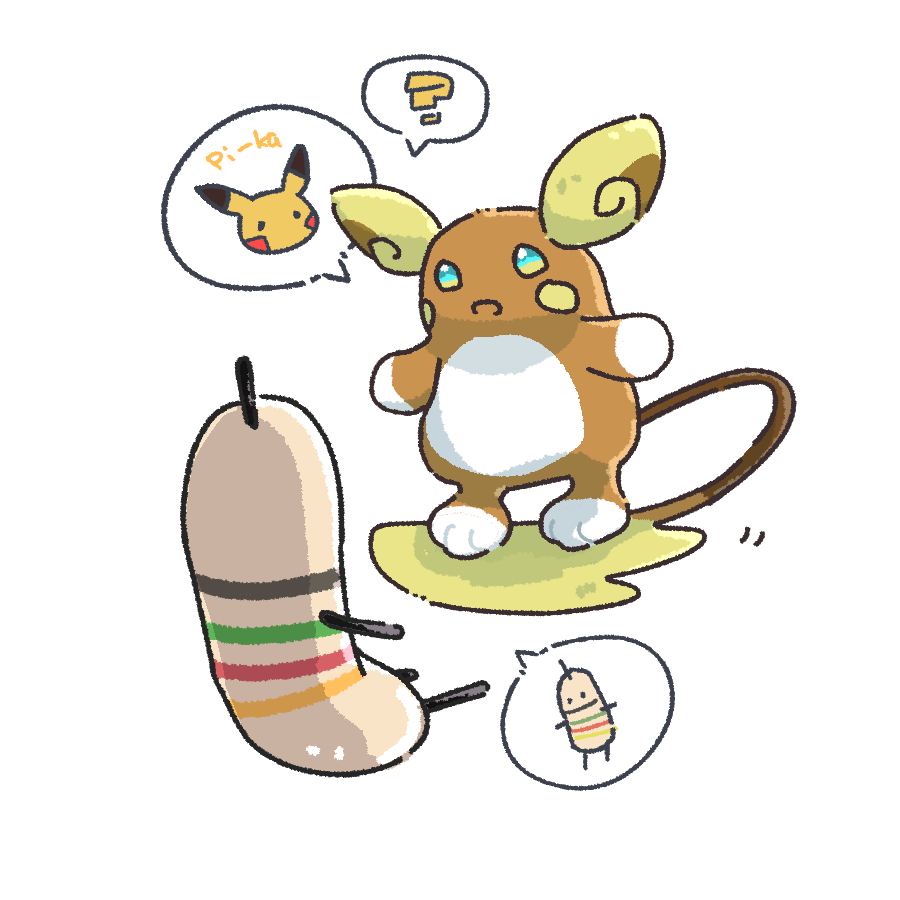
\includegraphics[width=0.7\linewidth]{figure/example.png}
        \caption{Example caption.}
        \label{fig:example}
    \end{figure}
    \note{
        Explain what the figure shows and what the audience should notice.
    }
\end{frame}

\begin{frame}{Example Table}
    \centering
    \begin{tabular}{lcc}
        \toprule
        Method & Metric 1 & Metric 2 \\
        \midrule
        A & 0.90 & 0.80 \\
        B & 0.93 & 0.85 \\
        C & 0.95 & 0.88 \\
        \bottomrule
    \end{tabular}
    \note{
        Highlight the most important comparison rather than reading the table.
    }
\end{frame}

% -----------------------------------------------------------------------------
% Section 3
% -----------------------------------------------------------------------------
\section{Conclusion}

\begin{frame}{Summary}
    \begin{itemize}
        \item Main takeaway 1
        \item Main takeaway 2
        \item Main takeaway 3
    \end{itemize}
    \note{
        Summarize the talk clearly and briefly.
    }
\end{frame}

\begin{frame}{Future Work}
    \begin{itemize}
        \item Open question 1
        \item Open question 2
        \item Possible extension 3
    \end{itemize}
    \note{
        Mention what remains unresolved and possible next steps.
    }
\end{frame}

\begin{frame}
    \centering
    {\Huge Thank you!}

    \vspace{1em}
    Questions?
    \note{
        Pause and invite questions.
    }
\end{frame}

\end{document}